\section{Programming using packet transactions}
\label{s:transactions}

To illustrate programming using packet transactions in \pktlanguage, we
describe how a programmer would express flowlet switching~\cite{flowlets} in
\pktlanguage (Figure~\ref{fig:flowlet}).  Flowlet switching is a load balancing
algorithm that harnesses the natural burstiness of TCP traffic to load balance
flowlets: sets of packets that are separated by a large enough interval in time
called the flowlet threshold.  This flowlet threshold is chosen to ensure that
packets from flowlets taking different paths are unlikely to arrive out of
order at a TCP receiver, which would degrade throughput.

\begin{figure}[!h]
\begin{small}
  \begin{lstlisting}[style=customc]
#define NUM_FLOWLETS      8000
#define FLOWLET_THRESHOLD 5
#define NUM_HOPS          10

struct Packet {
  int sport;
  int dport;
  int new_hop;
  int arrival;
  int next_hop;
  int idl; // index into last_time
  int ids; // index into saved_hop
};

int last_time [NUM_FLOWLETS] = {0};
int saved_hop [NUM_FLOWLETS] = {0};

void flowlet(struct Packet pkt) {
  pkt.new_hop = hash3(pkt.sport,
                      pkt.dport,
                      pkt.arrival)
                % NUM_HOPS;

  pkt.idl = hash2(pkt.sport,
                  pkt.dport)
            % NUM_FLOWLETS;

  pkt.ids = hash2(pkt.sport,
                  pkt.dport)
            % NUM_FLOWLETS;

  if (pkt.arrival -
      last_time[pkt.idl] >
      FLOWLET_THRESHOLD) {
    saved_hop[pkt.ids] = pkt.new_hop;
  }

  last_time[pkt.idl] = pkt.arrival;
  pkt.next_hop = saved_hop[pkt.ids];
}
\end{lstlisting}
\end{small}
\caption{Flowlet switching in \pktlanguage}
\label{fig:flowlet}
\end{figure}

\begin{figure*}[!t]
  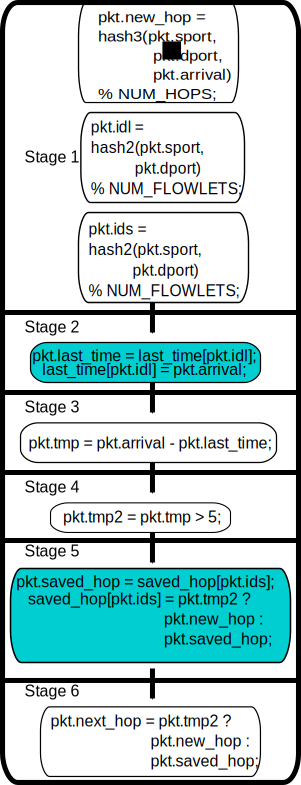
\includegraphics[width=\textwidth]{pipe.pdf}
  \caption{6-stage pipeline in \absmachine implementing flowlet switching}
  \label{fig:pipeline}
\end{figure*}

This example demonstrates the core language constructs in \pktlanguage. All
packet processing happens in the context of the packet transaction (the
function \texttt{flowlet} on line 17), a C function that takes a C struct as an
argument. The C struct declares the fields in a packet (lines 4--12) that can
be referenced by the function body (lines 17--39).  In addition, the function
body can reference state variables that represent persistent state stored on
the switch. These are declared as global variables at the program top level
(e.g. \texttt{last\_time} and \texttt{saved\_hop} on lines 14 and 15).

The semantics of the packet transaction function are to modify the packet that
it receives as argument in place until the end of the function body. Return
statements are forbidden; hence, execution will always end at the end of
the function body. The function body may also call out to opaque functions such
as \texttt{hash2} on lines 23 and 27 and \texttt{hash3} on line 18. These
represent hardware primitives provided by the abstract machine that have no
representation in \pktlanguage. The \pktlanguage compiler knows the signature
of opaque functions and uses these to infer dependencies, but doesn't know
anything about its implementation. Finally, the function body is written in a
constrained subset of C that excludes all iterative constructs. The function
body can include if and else-if statements, but all other control transfer
(break, goto, switch, return, and continue statements) is forbidden.

\pktlanguage forbids pointers and dynamic memory allocation. Arrays can be used
as state variables, but in a restriced form: for a given array, all accesses to
the array must use the same array index for a given packet. This restriction
simplifies the treatment of arrays in the compiler, while still being able to
express several data-plane algorithms of practical interest.

While these restrictions seem severe at first glance, they are required to
provide deterministic performance guarantees. Further, we show (\S\ref{s:eval})
that \pktlanguage can still express several data-plane algorithms  of practical
interest at a much higher level of abstraction than possible today.

When compiled to the \absmachine abstract machine (\S\ref{s:machine}), the
\pktlanguage compiler converts the code in Figure~\ref{fig:flowlet} into the
pipelined form shown in Figure~\ref{fig:pipeline}. Today, programmable switch
chips are programmed by manually specifying pipeline configurations resembling
Figure~\ref{fig:pipeline} using a language like P4 or an API such as Cavium's
XPliant SDK. This is a difficult and error-prone process~\cite{p4-semantics}.
Programming in \pktlanguage lets a compiler automate this process:
the user doesn't worry about hardware details such as pipeline stages and
concurrency within each stage.
